%%%%%%%%%%%%%%%%%%%%%%%%%%%%%%%%%%%%%%%%%%%%%%%%%%%%%%%%%%%%%%%%%%%%%%%%%%%%%%%
% Uni Duesseldorf
% Lehrstuhl fuer Datenbanken and Informationssysteme
% Vorlage fuer Bachelor-/Masterarbeiten
% Optimiert fuer den Original-Latex-Kompiler LATEX.EXE (LaTeX=>PS=>PDF)
% Version 1.4 - 2.3.2010
%%%%%%%%%%%%%%%%%%%%%%%%%%%%%%%%%%%%%%%%%%%%%%%%%%%%%%%%%%%%%%%%%%%%%%%%%%%%%%%

%%%%%%%%%%%%%%%%%%%%%%%%%%%%%%%%%%%%%%%%%%%%%%%%%%%%%%%%%%%%%%%%%%%%%%%%%%%%%%%
%%%%%%%%%%% BEGINN EINSTELLUNG FUER DIE ARBEIT. UNBEDINGT ERFORDERLICH! %%%%%%%
%%%%%%%%%%%%%%%%%%%%%%%%%%%%%%%%%%%%%%%%%%%%%%%%%%%%%%%%%%%%%%%%%%%%%%%%%%%%%%%
% Geben Sie Ihren Namen hier an
\newcommand{\bearbeiter}{Alina Elterman}

% Geben Sie hier den Titel Ihrer Arbeit an
\newcommand{\titel}{Game-theoretic Analysis of Strategyproofness in Cake-cutting Protocols}

% Geben Sie das Datum des Beginns and Ende der Bachelorarbeit ein
\newcommand{\beginndatum}{05. September 2011}
\newcommand{\abgabedatum}{05.~Dezember~2011}

% Geben Sie die Namen des Erst- and Zweitgutachters an
\newcommand{\erstgutachter}{Prof. Dr.~J\"org Rothe}
\newcommand{\zweitgutachter}{Prof. Dr.~Peter Kern}

% Falls Sie die Arbeit zweiseitig ausdrucken wollen,
% benutzen Sie die folgende Zeile mit
% \AN fuer zweiseitigen Druck
% \AUS fuer einseitigen Druck
\newcommand{\zweiseitig}{\AUS}

% Falls die Arbeit in englischer Sprache verfasst 
% werden soll, dann benutzen Sie die folgende Zeile mit
% englisch fuer englische Sprache
% deutsch fuer deutsche Sprache
\newcommand{\sprache}{englisch}
%%%%%%%%%%%%%%%%%%%%%%%%%%%%%%%%%%%%%%%%%%%%%%%%%%%%%%%%%%%%%%%%%%%%%%%%%%%%%%%%%
%%%%%%%%%%%%%%%%%%%%%%%%%%%%%%% ENDE EINSTELLUNGEN %%%%%%%%%%%%%%%%%%%%%%%%%%%%%%
%%%%%%%%%%%%%%%%%%%%%%%%%%%%%%%%%%%%%%%%%%%%%%%%%%%%%%%%%%%%%%%%%%%%%%%%%%%%%%%%%

% Die folgende Zeile NICHT EDITIEREN oder loeschen
% (Zum Ab�ndern der BA-Vorlage in eine MA-Vorlage muessen sie
% jedoch die Datei titelmakros1.tex selbst editieren.)
%%%%%%%%%%%%%%%%%%%%%%%%%%%%%%%%%%%%%%%%%%%%%%%%%%%%%%%%%%%
% Obere Titelmakros. Editieren Sie diese Datei nur, wenn
% Sie sich ABSOLUT sicher sind, was Sie da tun!!!
% (Z.B. zum Abaendern der BA-Vorlage in eine MA-Vorlage)
% Uni Duesseldorf
% Lehrstuhl fuer Datenbanken und Informationssysteme
% Version 2.2 - 2.3.2010
%%%%%%%%%%%%%%%%%%%%%%%%%%%%%%%%%%%%%%%%%%%%%%%%%%%%%%%%%%%
\newcommand{\AN}{twoside}
\newcommand{\AUS}{}
%\newcommand{\englisch}{}
%\newcommand{\deutsch}{\usepackage[german]{babel}}

%% Die folgenden auskommentierten Optionen dienen der automatischen
%% Erkennung des Latex-Kompilers und dem Setzen der davon abh�ngigen
%% Einstellungen. Bei Problem z.B. mit dem Einbinden von verschiedenen
%% Grafiktypen bei Verwendung von PdfLatex oder Latex, einfach die
%% verschiedenen \usepackage(s) ausprobieren. (Mit diesen Einstellungen
%% funktionierte diese Vorlage bei der Verwenundg von latex.exe als
%% Kompiler bei den meisten Studierenden.)

%\newif\ifpdf \ifx\pdfoutput\undefined
%\pdffalse % we are not running pdflatex
%\else
%\pdfoutput=1 % we are running pdflatex
%\pdfcompresslevel=9 % compression level for text and image;
%\pdftrue \fi

\documentclass[11pt,a4paper, \zweiseitig]{article}



%\usepackage[iso]{umlaute}
%\usepackage[latin1]{inputenc}
\usepackage{palatino} % palatino Schriftart
%\usepackage{makeidx} % um ein Index zu erstellen
\usepackage{tocbibind}
\usepackage[T1]{fontenc} %fuer richtige Trennung bei Umlauten
\usepackage{fancybox} % fuer die Rahmen
\usepackage{shortvrb}
\usepackage{ifthen}
%\ifthenelse{\equal{\sprache}{deutsch}}{\usepackage[ngerman]{babel}}{}
\usepackage[utf8]{inputenc}
\usepackage{lmodern} 
\usepackage{amsmath}
\usepackage{oldgerm}
\usepackage{amssymb}
\usepackage{pdfpages}
\usepackage{hyperref}
%\usepackage{fancyheadings}
\usepackage{fancyhdr}
\usepackage{amsfonts}
\usepackage{amsthm}
\usepackage{color}
%\usepackage{stmaryrd}
\usepackage{graphicx}
\usepackage{nomencl}
\usepackage[normalem]{ulem} 
\usepackage{verbatim}
\usepackage{ulsy}
\usepackage{tikz}
\usepackage{pgf}
\usepackage{bbding}
\usepackage{nicefrac}
\usepackage{multirow}
\usetikzlibrary{arrows,automata,petri,shapes,snakes}


\newcommand{\markup}[1]{\uline{#1}}
% Befehl umbenennen in abk
\let\abk\nomenclature

\usepackage{a4wide} % ganze A4 Weite verwenden

%\ifpdf
%\usepackage[pdftex,xdvi]{graphicx}
%\usepackage{thumbpdf} %thumbs fuer Pdf
%\usepackage[pdfstartview=FitV]{hyperref} %anklickbares Inhaltsverzeichnis
%\else
%\usepackage[dvips,xdvi]{graphicx}
%\usepackage{hyperref} %anklickbares Inhaltsverzeichnis
%\fi

%%%%%%%%%%%%%%%%%%%%%%% Massangaben fuer die Arbeit %%%%%%%%%%%%%%%
\setlength{\textwidth}{15cm}

\setlength{\oddsidemargin}{35mm}
\setlength{\evensidemargin}{25mm}

\addtolength{\oddsidemargin}{-1in}
\addtolength{\evensidemargin}{-1in}

%\makeindex
% Umgebungen f"ur S�tze usw.
\newtheorem{bemerkung*}{Comment}
\newtheorem{defi}{Definition}
\newtheorem{defi*}{Definition}
\newtheorem{bezeichnungen}{Remark}
\newtheorem{fakt}{Fact}
\newtheorem{beispiel}{Example}
\newtheorem{bsp}{Example}
\newtheorem{beispiel*}{Example}
\newtheorem{satz}{Theorem}
\newtheorem{satz*}{Theorem}
\newtheorem{lem}{Theorem}
\newtheorem{protokoll*}{Protocol}
\newtheorem{idee}{Idea}
\newtheorem{corollary}{Corollary}

%definition of new commands
\newcommand{\DGEF}{\text{\textbf{DGEF}}}
\newcommand{\vsp}{\vspace{3mm}}
\newcommand{\impl}[1]{\overset{\text{#1}}{\implies}}
\newcommand{\notimplleft}[1]{\overset{\text{#1}}{\not\Leftarrow}}

\begin{document}

%\setcounter{secnumdepth}{4} %Nummerieren bis in die 4. Ebene
%\setcounter{tocdepth}{4} %Inhaltsverzeichnis bis zur 4. Ebene

\pagestyle{headings}
\thispagestyle{empty}
\sloppy % LaTeX ist dann nicht so streng mit der Silbentrennung
%\MakeShortVerb{\�}

\parindent0mm
\parskip0.5em


{
\textwidth170mm 
\oddsidemargin30mm 
\evensidemargin30mm 
\addtolength{\oddsidemargin}{-1in}
\addtolength{\evensidemargin}{-1in}

\parskip0pt plus2pt

% Die Raender muessen eventuell fuer jeden Drucker individuell eingestellt
% werden. Dazu sind die Werte fuer die Abstaende `\oben' und `\links' zu
% aendern, die von mir auf jeweils 0mm eingestellt wurden.

%\newlength{\links} \setlength{\links}{10mm}  % hier abzuaendern
%\addtolength{\oddsidemargin}{\links}
%\addtolength{\evensidemargin}{\links}

\begin{titlepage}
\vspace*{-1.5cm}
  \raisebox{17mm}{
    \begin{minipage}[t]{70mm}
      \begin{center}
        %\selectlanguage{german}
        {\Large INSTITUT FÜR INFORMATIK\\}
        {\normalsize
          Lehrstuhl für Komplexitätstheorie und Kryptologie
\\
        }
        \vspace{3mm}
        {\small Universitätsstr. 1 \hspace{5ex} D--40225 Düsseldorf\\}
     \end{center}
    \end{minipage}
  }
  \hfill
  
\includegraphics[width=130pt]{bilder/HHU_Logo}
  \vspace{14em}

% Titel
  \begin{center}
      	\baselineskip=55pt
    	\textbf{\huge \titel}
  	 	\baselineskip=0 pt
   \end{center}

  %\vspace{7em}

\vfill

% Autor
  \begin{center}
    \textbf{\Large
      \bearbeiter
    }
  \end{center}

  \vspace{35mm}
 
% Pr�fungsordnungs-Angaben
  \begin{center}
    %\selectlanguage{german}
    
%%%%%%%%%%%%%%%%%%%%%%%%%%%%%%%%%%%%%%%%%%%%%%%%%%%%%%%%%%%%%%%%%%%%%%%%%
% Ja, richtig, hier kann die BA-Vorlage zur MA-Vorlage gemacht werden...
%%%%%%%%%%%%%%%%%%%%%%%%%%%%%%%%%%%%%%%%%%%%%%%%%%%%%%%%%%%%%%%%%%%%%%%%%
    {\Large Bachelorarbeit}

    \vspace{2em}

    \begin{tabular}[t]{ll}
      Beginn der Arbeit:& \beginndatum \\
      Abgabe der Arbeit:& \abgabedatum \\
      Gutachter:         & \erstgutachter \\
                         & \zweitgutachter \\
    \end{tabular}
  \end{center}

\end{titlepage}

}

%%%%%%%%%%%%%%%%%%%%%%%%%%%%%%%%%%%%%%%%%%%%%%%%%%%%%%%%%%%%%%%%%%%%%
\clearpage
\begin{titlepage}
  ~                % eine leere Seite hinter dem Deckblatt
\end{titlepage}
%%%%%%%%%%%%%%%%%%%%%%%%%%%%%%%%%%%%%%%%%%%%%%%%%%%%%%%%%%%%%%%%%%%%%
\clearpage
\begin{titlepage}
\vspace*{\fill}

\section*{Erklärung}

%%%%%%%%%%%%%%%%%%%%%%%%%%%%%%%%%%%%%%%%%%%%%%%%%%%%%%%%%%%
% Und hier ebenfalls ggf. BA durch MA ersetzen...
%%%%%%%%%%%%%%%%%%%%%%%%%%%%%%%%%%%%%%%%%%%%%%%%%%%%%%%%%%%

Hiermit versichere ich, dass ich diese Bachelorarbeit
selbstständig verfasst habe. Ich habe dazu keine anderen als die
angegebenen Quellen und Hilfsmittel verwendet.

\vspace{25 mm}

\begin{tabular}{lc}
Düsseldorf, den \abgabedatum \hspace*{2cm} & \underline{\hspace{6cm}}\\
& \bearbeiter
\end{tabular}

\vspace*{\fill}
\end{titlepage}

%%%%%%%%%%%%%%%%%%%%%%%%%%%%%%%%%%%%%%%%%%%%%%%%%%%%%%%%%%%%%%%%%%%%%
% Leerseite bei zweiseitigem Druck
%%%%%%%%%%%%%%%%%%%%%%%%%%%%%%%%%%%%%%%%%%%%%%%%%%%%%%%%%%%%%%%%%%%%%

\ifthenelse{\equal{\zweiseitig}{twoside}}{\clearpage\begin{titlepage}
~\end{titlepage}}{}

%%%%%%%%%%%%%%%%%%%%%%%%%%%%%%%%%%%%%%%%%%%%%%%%%%%%%%%%%%%%%%%%%%%%%
\clearpage
\begin{titlepage}

\section*{\ifthenelse{\equal{\sprache}{deutsch}}{Zusammenfassung}{Abstract}}


%%%%%%%%%%%%%%%%%%%%%%%%%%%%%%%%%%%%%%%%%%%%%%%%%%%%%%%%%%%%%%%%%%%%%%%%%%%%%%%%%
%%%%%%%%%%%%%%%%%%%%%%%%%%%% BEGINN ZUSAMMENFASSUNG %%%%%%%%%%%%%%%%%%%%%%%%%%%%%
%%%%%%%%%%%%%%%%%%%%%%%%%%%%%%%%%%%%%%%%%%%%%%%%%%%%%%%%%%%%%%%%%%%%%%%%%%%%%%%%%
%\begin{enumerate}
%\item What is the problem?
%\item Why interesting?
%\item How to solve?
%\item What is the result?
%\end{enumerate}

%%%%%%%%%%%%%%%%%%%%%%%%%%%%%%%%%%%%%%%%%%%%%%%%%%%%%%%%%%%%%%%%%%%%%%%%%%%%%%%%%
%%%%%%%%%%%%%%%%%%%%%%%%%%%%% ENDE ZUSAMMENFASSUNG %%%%%%%%%%%%%%%%%%%%%%%%%%%%%%
%%%%%%%%%%%%%%%%%%%%%%%%%%%%%%%%%%%%%%%%%%%%%%%%%%%%%%%%%%%%%%%%%%%%%%%%%%%%%%%%%

% Die folgende Zeile NICHT EDITIEREN oder loeschen
%%%%%%%%%%%%%%%%%%%%%%%%%%%%%%%%%%%%%%%%%%%%%%%%
% Untere Titelmakros. Editieren Sie diese Datei nur, wenn Sie sich
% ABSOLUT sicher sind, was Sie da tun!!!
%%%%%%%%%%%%%%%%%%%%%%%%%%%%%%%%%%%%%%%%%%%%%%%
\vspace*{\fill}
\end{titlepage}

%%%%%%%%%%%%%%%%%%%%%%%%%%%%%%%%%%%%%%%%%%%%%%%%%%%%%%%%%%%%%%%%%%%%%
% Leerseite bei zweiseitigem Druck
%%%%%%%%%%%%%%%%%%%%%%%%%%%%%%%%%%%%%%%%%%%%%%%%%%%%%%%%%%%%%%%%%%%%%
\ifthenelse{\equal{\zweiseitig}{twoside}}
  {\clearpage\begin{titlepage}~\end{titlepage}}{}
%%%%%%%%%%%%%%%%%%%%%%%%%%%%%%%%%%%%%%%%%%%%%%%%%%%%%%%%%%%%%%%%%%%%%
\clearpage 
\tableofcontents
\thispagestyle{empty}
%\enlargethispage{\baselineskip}
\clearpage \setcounter{page}{1}
%%%%%%%%%%%%%%%%%%%%%%%%%%%%%%%%%%%%%%%%%%%%%%%%%%%%%%%%%%%%%%%%%%%%%
% Leere Seite, falls Inhaltsverzeichnis mit ungerader Seitenzahl und 
% doppelseitiger Druck
%%%%%%%%%%%%%%%%%%%%%%%%%%%%%%%%%%%%%%%%%%%%%%%%%%%%%%%%%%%%%%%%%%%%%
\ifthenelse{ \( \equal{\zweiseitig}{twoside} \and \not \isodd{\value{page}} \)}
	{\pagebreak \thispagestyle{empty} \cleardoublepage}{\clearpage}



%%%%%%%%%%%%%%%%%%%%%%%%%%%%%%%%%%%%%%%%%%%%%%%%%%%%%%%%%%%%%%%%%%%%%
%%%%%%%%%%%%%%%%%%%%%%%%% BEGINN TEXTTEIL %%%%%%%%%%%%%%%%%%%%%%%%%%%
%%%%%%%%%%%%%%%%%%%%%%%%%%%%%%%%%%%%%%%%%%%%%%%%%%%%%%%%%%%%%%%%%%%%%
\section{Introduction}
Strategic play, cheating, incentive compatible, risk aversion, truthfulness, strategyproof and a lot more. All of them are keywords of whether an algorithm can resist the actions of selfish players and their greedyness.
%\\
%\newline
%Cake-cutting is part of interdisciplinary fields like economics, mathematics, operations research, political and computer science. Game theory is fulfilling the same property. Except for this fact, they have hardly something in common. While cake cutting is about fair division of a heterogeneous divisible good, where the studies are especially concentrated on types of fairness, game theory studies the strategies people use when making decisions.\\
%The role of strategies has not been widely researched yet in the context of cake cutting. But their importance is indisputable, with respect to fairness. Imagine the following situation:
%Example Cost Sharing from Algorithmic GT Noam Nissan chap. 15
%\begin{itemize}
%\item{division of sports tickets, health resources, computer networking resources, voting power, intellectual property licenses, costs for environmental improvements, etc}
%\item{formalize fairness, including max-min fairness, proportional fairness, envy-free fairness, etc. which may or may not lead to stable allocations in the sense of say Nash Equilibrium, or strong Nash Equilibrium}
%\end{itemize}
%Es werden Auswirkungen von nicht ehrlichen Strategien auf die Gerechtigkeit von Protokollen betrachtet. Der approach der Neidfreiheit ist zu stark, da kein finite bounded Protokoll f"ur n >3 (>4 f"ur allgemein) bekannt ist. Dagegen w"are der approach der Proportionaltit"at zu schwach, $\dots$. Das notwendige Mittelmaß liefert der DGEF und so fällt der Focus dieser Arbeit auf die Möglichkeit den DGEF eines Protokolles durch unehrliche Strategien zu erhöhen. Die Analyse erfolgt mittels Spieltheorie.\\
%\newline
%$\cdot$ Able to show that the only strategy promising a fair share is the recommended one.
\pagebreak
%%%%%%%%%%%%%%%%%%%%%%%%%%%%%%%%%%%%%%%%%%%%%%%%%%%%%%%%%%%%%%%%%%%%%%%%%%%%%%%%%%%%%%%%%%%%%%%%%%%%%%%%%%%%%%%%
%%%%%%%%%%%%%%%%%%%%%%%%%%%%%%%%%%%%%%%%%%%%%%%%%%%%%%%%%%%%%%%%%%%%%%%%%%%%%%%%%%%%%%%%%%%%%%%%%%%%%%%%%%%%%%%%
%%%%%%%%%%%%%%%%%%%%%%%%%%%%%%%%%%%%%%%%%%%%%%%%%%%%%%%%%%%%%%%%%%%%%%%%%%%%%%%%%%%%%%%%%%%%%%%%%%%%%%%%%%%%%%%%
\subsection{Related Work}
%In the field of cake-cutting the idea of counting envy- and envy-free-relations was introduced by Brams, Jones and Klamler (2007) mostly in the egalitarian way. It was edited to the utalitarian perspective and expanded by Lindner and Rothe (2009). The history and the scope of work done in other fields can be found in detail in the second work.\\
%\newline
%\begin{tabular}{cll}
%Truthfulness:&
%$\cdot$ GT:&\\&
%$\cdot$ MD:&\\&
%$\cdot$ SC:&\\&
%$\cdot$ CC(FD):&Ariel and Tamuz weakened the basic assumptions\\&&of cake-cutting and so only analysed special cases.\\&
%$\cdot$ CC(MARA):&A lot of papers e.g. Lipton, Markakis $\dots$\\
%\end{tabular}
\pagebreak
%%%%%%%%%%%%%%%%%%%%%%%%%%%%%%%%%%%%%%%%%%%%%%%%%%%%%%%%%%%%%%%%%%%%%%%%%%%%%%%%%%%%%%%%%%%%%%%%%%%%%%%%%%%%%%%%
%%%%%%%%%%%%%%%%%%%%%%%%%%%%%%%%%%%%%%%%%%%%%%%%%%%%%%%%%%%%%%%%%%%%%%%%%%%%%%%%%%%%%%%%%%%%%%%%%%%%%%%%%%%%%%%%
%%%%%%%%%%%%%%%%%%%%%%%%%%%%%%%%%%%%%%%%%%%%%%%%%%%%%%%%%%%%%%%%%%%%%%%%%%%%%%%%%%%%%%%%%%%%%%%%%%%%%%%%%%%%%%%%
\section{Preliminaries}
\subsection{Preliminaries of Game Theory}
In this chapter some basic concepts from game theory are described and directly applied to the cake-cutting problem. The best fitting game-theoretic model is called bayesian game. The development to this result and use of the associated solution concepts is described.\\
Game theory can be seen as a tool for describing interaction in lifes processes. The occuring problems can be simulated by games.  
%Non-cooperated game theory is about single selfish players, and in cooperated the main focus is on forming coalitions. For computer scientists especially the algorithmic game theory is of major interest, because $\dots$. 
\begin{defi}{\textbf{(Game)}}\\
A \underline{non-cooperative (strategic) game} $\Gamma=(P_n,S,u)$ consists of the set of players $P_n$ , the set of strategies $S$ and the set of utility functions (pay-off) of all players $u_i$.
\begin{itemize}
\item Each player in the set $P_n=\{p_1,\cdots,p_n\}$ behave selfish and rational.
\end{itemize}
\end{defi}

\begin{defi}{\textbf{(Strategies)}}
dominant, dominated, best response
\end{defi}
\begin{defi}{\textbf{(Pay-off function)}}
A Egalitarian and utiletarian
\end{defi}
\textbf{Classes of Special Games}\\
\begin{defi}{\textbf{(Zero-Sum Game)}}
A 
\end{defi}
Cutting a cake is a non-zero-sum game, since it allows players to get better off than 1/n-th. An exception is a homogenius cake, then the valuations over the cake are equal and the the game zero-sum.\\
\newline
\begin{defi}{\textbf{(Bayesian Game)}}
A 
\end{defi}
A game can be represented in normal or in extended form.
 
%%%%%%%%%%%%%%%%%%%%%%%%%%%%%%%%%%%%%%%%%%%%%%%%%%%%%%%%%%%%%%%%%%%%%%%%%%%%%%%%%%%%%%%%%%%%%%%%%%%%%%%%%%%%%%%%
%%%%%%%%%%%%%%%%%%%%%%%%%%%%%%%%%%%%%%%%%%%%%%%%%%%%%%%%%%%%%%%%%%%%%%%%%%%%%%%%%%%%%%%%%%%%%%%%%%%%%%%%%%%%%%%%
%%%%%%%%%%%%%%%%%%%%%%%%%%%%%%%%%%%%%%%%%%%%%%%%%%%%%%%%%%%%%%%%%%%%%%%%%%%%%%%%%%%%%%%%%%%%%%%%%%%%%%%%%%%%%%%%
\subsection{Preliminaries of Cake-cutting}
\subsubsection{Basics}
First, it is necessary to define the components of cake-cutting. Example \ref{bsp1} describes the problem.
%
\begin{bsp}
\label{bsp1}
Cocke, Younger and Kasami have a cheese-chocolate-straberry-cake. 
\end{bsp}
Now, what exactly is cake-cutting about? First of all, it involves a discrete set of $n \in \mathbb{N}$ agents (or players ) $P_n=\{p_1,\cdots,p_n\}$. It is assumed that each of them wants to get as much as possible of the divided good. The goal is to allocate it in a manner that each player is satisfied. The allocation of a single, divisible and heterogeneous good is included in the consideration of this work.\\ 
	\begin{figure}[h]
		\centering
 		 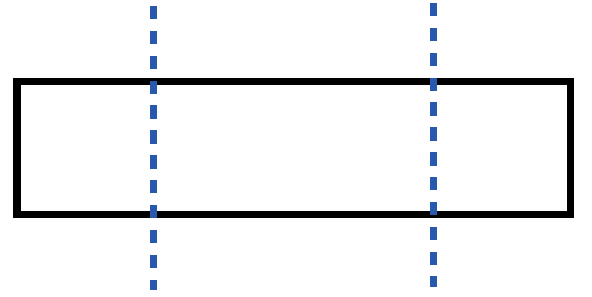
\includegraphics[width=130pt]{kek.pdf}
   \caption{Cake}Example for a visualisation of a cake and two cuts
  	 \end{figure}
For the visualization it is common to use a rectangular cake. The division is performed by parallel cuts. The cake $X$ is represented by the unit interval $I=[0,1] \subseteq \mathbb{R}$. Each disjoint subinterval $I'\subseteq I$ or a union of such subintervals $$\sideset{}{ }\bigcup\limits_{m\in\mathbb{N}}I_m$$
with $I_m\subseteq I$ is called a bundle (or piece). The bundle of the cake, which the player $p_i$ receives is denoted as $X_i$. The state is called an \underline{allocation}, when all bundles of the cake are owned by players. Each piece has a public length, which can be computed as the sum of all border differences, and the private value of each player.\\

Every player $p_i\in P_n$ has a \underline{valuation function (valuation)} $v_i:\{X'|X' \subseteq X\} \rightarrow [0,1]$ on the cake $X$ with the following properties:
\begin{enumerate}
\item Non-negativity: $v_i(C)\geq 0$ for all $C\subseteq [0,1].$
\item Normalisation: $v_i(\emptyset)=0$ and $v_i([0,1])=1.$
\item Additivity: $v_i(C \cup C')=v_i(C)+v_i(C')$ for disjoint
$C,C'\subseteq [0,1].$\footnote{Monotonicity: If $C' \subseteq C$ then $v_i(C') \leq v_i(C)$ follows from additivity, because for the assumption $C' \subseteq C$ and $A:=C\backslash C'$: $v_i(C)=v_i(A\cup C')=v_i(A)+v_i(C')=\underbrace{v_i(C\backslash C')}_{\geq 0}+v_i(C')\geq v_i(C').$}
\item Divisibility: For all $C\subseteq [0,1]$ and all $\alpha \in
\mathbb{R}$, $0\leq \alpha \leq 1$, exists a $B\subseteq C$, so that
$v_i(B)=\alpha \cdot v_i(C).$
\item  $v_i$ is continuous: If $0<x<y\leq 1$ with $v_i([0,x])=\alpha$ and
$v_i([0,y])=\beta$, then for every $\gamma \in [\alpha,\beta]$ there exists a $z \in [x,y]$ so that $v_i([0,z])=\gamma.$
\item Non-atomic:  $v_i([x,x])=0$ for all $x\in [0,1].$
\end{enumerate}
%%%%%%%%%%%%%%%%%%%%%%%%%%%%%%%%%%%%%%%%%%%%%%%%%%%%%%%%%%%%%%%%%%%%%%%%%%%%%%%%%%%%%%%%%%%%%%%%%%%%%%%%%%%%%%%%
%%%%%%%%%%%%%%%%%%%%%%%%%%%%%%%%%%%%%%%%%%%%%%%%%%%%%%%%%%%%%%%%%%%%%%%%%%%%%%%%%%%%%%%%%%%%%%%%%%%%%%%%%%%%%%%%
%%%%%%%%%%%%%%%%%%%%%%%%%%%%%%%%%%%%%%%%%%%%%%%%%%%%%%%%%%%%%%%%%%%%%%%%%%%%%%%%%%%%%%%%%%%%%%%%%%%%%%%%%%%%%%%%
\textbf{Different Types of Fairness}\\
\newline
Especially the fairness plays an important role in fair division. But how is fairness defined? It can be seen as a valuation criteria of an allocation, which can be normalized and gives a possibility to compare different allocations. Usually the fairness criteria are distinguished between the following:
\begin{defi}{\textbf{(Proportional or Simple Fair)}}
\newline An allocation is \underline{proportional (simple fair)}, if
$v_i(X_i) \geq 1/n$ for each player $p_i \in P_N$.
\end{defi}
\begin{defi}{\textbf{(Envy-Freeness)}}
\newline An allocation is \underline{envy-free}, if $v_i(X_i) \geq
v_i(X_j)$ for each couple of players $p_i, p_j \in P_N$.
\end{defi}
%\begin{defi}{\textbf{(Equity)}}
%\newline An allocation is \underline{equitable}, if $v_i(X_i) =
%\alpha$ for each player $p_i \in P_N$ and $0 \leq \alpha \leq 1$ \footnote{ If $\alpha = 1/n$ the allocation is called \underline{exact}.}.
%\end{defi}
%
\textbf{Correlation between the Fairness-Properties}
\begin{lem}
For all allocations:
\begin{enumerate}
\item Every envy-free allocation is proportional.
\item For two players an allocation is envy-free iff it is proportional.
\end{enumerate}
\end{lem}
\begin{proof}
\begin{enumerate}
\item Proof by contradiction:\\ Assume $A$ is an envy-free allocation, but not proportional. From envy-freeness follows $v_i(X_i) \geq v_i(X_j)$ for each couple of players $p_i, p_j \in P_N$ and so each player has at least as much cake as each other player. Hereby each player owns at least as much as $(n-1)$ other players and so at least $1/n$. The allocation $A$ is proportional. %$\lightning$ 
\\Therefore all envy-free allocations are proportional.
\item ''$\Rightarrow$'' For two players an allocation is proportional if each player has at least the half ot the cake. So the first player thinks the second player got at most half of the cake and vice versa. They would not envy each other.\\ ''$\Leftarrow$'' Follows from part 1.\\
\end{enumerate}
\end{proof}
A slighly different criteria to valuate the performance of an allocation is the efficiency. The correlation between the fairness criterion and efficiency can be found in \cite{eff}. 
\begin{defi}{\textbf{(Efficiency)}}
\newline An allocation $A=\{X_1,\dots, X_n\}$ is \underline{efficient (Pareto optimal)} if there is no other allocation $A'=\{X'_1,\dots, X'_n\}$ such that $v_i(X_i)\leq v_i(X'_i)$ for all players $p_i \in P_n$ and for at least one player the inequality is strict.
\end{defi}
 
\begin{lem}
For all allocations:
	\begin{enumerate}
		\item Proportionality does not imply efficiency.
		\item Efficiency does not ensure fairness.
	\end{enumerate}
\end{lem}

\begin{proof}
	\begin{enumerate}
		\item Imagine the following allocation with three players:
		\begin{center}
		\begin{tabular}{c|ccc}
		& $X_1$& $X_2$& $X_3$\\
		\hline
		$p_1$ & \textcolor{blue}{$\frac{1}{3}$} & $\frac{1}{2}$ & $\frac{1}{6}$\\ \\
  $p_2$ & $\frac{1}{3}$ & \textcolor{blue}{$\frac{1}{3}$} & $\frac{1}{3}$\\ \\
  $p_3$ & $0$ & $\frac{7}{18}$ & \textcolor{blue}{$\frac{11}{18}$}
 		\end{tabular}	 
 		\end{center}
		
		This allocation is obviously proportional, since $v_i(X_i) \geq 1/3$ for all $i \in \{1,2,3\}$. It is not efficient, because if the players $p_1$ and $p_2$ exchange their pieces, $p_2$ would get more of the cake and $p_1$ would not get less.
		\item Allocating the whole cake to one player is efficient, but definitely not proportional and therefore not envy-free.
	\end{enumerate}
\end{proof}
In \cite{brams2} the authors showed a general argument that no finite bounded procedure can exist for such an allocation that is both, proportional and efficient at the same time.
%%%%%%%%%%%%%%%%%%%%%%%%%%%%%%%%%%%%%%%%%%%%%%%%%%%%%%%%%%%%%%%%%%%%%%%%%%%%%%%%%%%%%%%%%%%%%%%%%%%%%%%%%%%%%%%%
%%%%%%%%%%%%%%%%%%%%%%%%%%%%%%%%%%%%%%%%%%%%%%%%%%%%%%%%%%%%%%%%%%%%%%%%%%%%%%%%%%%%%%%%%%%%%%%%%%%%%%%%%%%%%%%%
%%%%%%%%%%%%%%%%%%%%%%%%%%%%%%%%%%%%%%%%%%%%%%%%%%%%%%%%%%%%%%%%%%%%%%%%%%%%%%%%%%%%%%%%%%%%%%%%%%%%%%%%%%%%%%%%
\subsubsection{Strategyproofness}
In the wide spectrum of literature different definitions and specifications about the honesty of players occur. Since the origin is game-theoretic and the main research is done in mechanism design, which is a part of game theory, the most results are from there. Nevertheless some definitions adapted to cake-cutting exist.\\
In practice players are selfish and try to increase the value of their bundle. In order to do so, they may report false valuations on parts of the cake. The goal is to prevent this.
\begin{defi}{\textbf{(Risk Aversion)}}(\cite{brams})
A player is \underline{risk averse} if he or she will never choose a strategy that may yield a more valuable piece of cake if it entails the possibility of getting less than a piece of a guaranteed size.
\end{defi}
\begin{defi}{\textbf{(Strategyproofness of a Proportinal Protocol)}}(\cite{lindner:degrees})\\
A proportional cake-cutting protocol is said to be \underline{strategyproof for risk averse players} if a cheating player is no longer guaranteed a proportional share, whereas all other players (provided they play truthfully) are still guaranteed to receive their proportional share.
\end{defi}
%\textbf{Notice:} The actions of a player do not harm any of the other players.
\begin{defi}{\textbf{(Truthfully)}}
An allocation is \underline{truthful} if the value of the cake obtained by a player by reporting false is not greater than by reporting the truth.
\end{defi}

\begin{defi}{\textbf{(Strategyproofness)}}(\cite{pie})\\
A procedure is \underline{strategyproof} if no player has a strategy that dominates his true value function.
\end{defi}

A stronger condition from social choice literature:

\begin{defi}{\textbf{(Strategyproofness)}}(\cite{why})\\
A procedure is \underline{strategyproof} if the true value function dominates every other strategy.
\end{defi}

%Assume the statement is true, where each player acts truthfully by following his best strategy, which yields to a maximum possible allocation for a player ''$\Leftrightarrow$'' Nash-equilibrium. But there is a problem, like \cite{malik} detected no known algorithm can fulfill this promise. The appealing alternative is the guarantee of a fair share for telling the truth.\\
In order to prevent misunderstandings in this paper it will be called strong strategyproofness. It can be shown, that cake-cutting is not able to fulfill the strong strategyproofness criteria. The following example is similar to the one in \cite{chen:truth}.\\

\begin{bsp}
John Warner Backus and Peter Naur are celebrating and Donald E. Knuth has brough a huge marzipan cake with an enormous cherry on top. John loves cherries and hate marzipan, and Peter is just very hungry. The pioneers of computer science apply cut $\&$ choose \footnote{see next page}. Peter is the cutter, and his best strategy is to separate the cake from the cherry. And if Peter would have the fully knowledge (which should be no problem for the strategyproofness in \cite{why}) about the valuations of John, he would always benefit by lying and so this algorithm is not strong strategyproof.  
\end{bsp}
%\newline
%The question arise, whether a protocol can force truthfulness.\\
%An example will be the following case where $n$ players cut the cake in pieces with $v_i(X_i)=\frac{1}{n}$ and then allocate them randomly to the players.\\
%\newline

%%%%%%%%%%%%%%%%%%%%%%%%%%%%%%%%%%%%%%%%%%%%%%%%%%%%%%%%%%%%%%%%%%%%%%%%%%%%%%%%%%%%%%%%%%%%%%%%%%%%%%%%%%%%%%%%
%%%%%%%%%%%%%%%%%%%%%%%%%%%%%%%%%%%%%%%%%%%%%%%%%%%%%%%%%%%%%%%%%%%%%%%%%%%%%%%%%%%%%%%%%%%%%%%%%%%%%%%%%%%%%%%%
%%%%%%%%%%%%%%%%%%%%%%%%%%%%%%%%%%%%%%%%%%%%%%%%%%%%%%%%%%%%%%%%%%%%%%%%%%%%%%%%%%%%%%%%%%%%%%%%%%%%%%%%%%%%%%%%
\textbf{Different Types of Protocols}\\
\newline
It is very important to understand the types, structure and design of protocols, which will be analysed in this paper.\\
\newline
Informal: (Algorithm)
\newline In mathematics, computer science and related subjects, an
\underline{algorithm} is an effective method for solving a problem, which can be denoted as a finite set of sequences.
\begin{defi}{\textbf{(Protocol (Cake-Cutting-Protocol))}}
\newline A \underline{protocol (cake-cutting-protocol)} is an adaptive algorithm with a fixed number of players and the following properties:
\begin{itemize}
\item{It consists of rules and strategies.\\ \underline{Rules} are requirements, which have to be followed by the players without knowledge of their valuations.\\
\underline{Strategies} are recommendations, which can be followed for getting the guaranteed fair share.}
\item{If a player does not follow the strategy of a protocol, he looses his guarantee to get a fair piece of cake after a fixed number of steps. His actions do not harm the other players.}
\item Each player should be able to cut the cake at a specific moment independent of other players.
\item The protocol has no information about the valuation of the players, except of those it got from the steps before. It can not prove whether a player follows the strategy of the protocol.
\end{itemize}
\end{defi}
\begin{bsp}
(Representation idea taken from \cite{Barbanel})\\
\begin{tabular*}{\textwidth}[]{|@{\extracolsep{\fill}}ccc|}
\hline
\hline
&\textbf{Cut $\&$ choose for $n=2$}&\\
\end{tabular*}
\begin{tabular*}{\textwidth}{|@{\extracolsep{\fill}}l|c|r|}
\hline
\textbf{Rules}& \textbf{Player $p_1$ strategy}& \textbf{Player $p_2$ strategy}\\
\hline
1. Player $p_1$ partition &Partition $X$ into two&\\
the cake $X$ into two&pieces of equal size&\\
pieces $\{X',X-X'\}$&&\\
\hline
2. Player $p_2$ chooses&&Choose the bigger piece\\
one piece&&\\
\hline
3. Player $p_1$ get the &&\\remaining piece&&\\
\hline
\end{tabular*}
\end{bsp}
\begin{satz}
Cut $\&$ choose is strategyproof.
\end{satz}
\begin{proof}
\textbf{Options for not following the recomended strategy:}
\begin{itemize}
\item Player $p_2$ takes the smaller piece. This can not be his intention, because then he is less satiesfied after the basic assumption.
\item Player $p_1$ cuts the cake into two not equal pieces. The chance to get less is equal to the chance to get more of the cake. In stochastic terms it means, that the expected value at the end of the allocation will be in the honest case: $$ \frac{1}{2} \cdot \frac{1}{2}+\frac{1}{2} \cdot \frac{1}{2}=\frac{1}{2} $$ and in the dishonest case: $$ \frac{1}{2} \cdot X' +\frac{1}{2} \cdot (X-X') =\frac{1}{2} \cdot \underbrace{X}_{=1}=\frac{1}{2}$$ According to the definition of truthfulness in the case with equal outcomes the player would stay honest.
\end{itemize}
\end{proof}

\begin{defi}{\textbf{(Proportional/ Envy-Free Protocol)}}\\
A cake-cutting \underline{protocol} is called \underline{proportional} or \underline{envy-free}, if independent of the players' valuation, each allocation is proportional or envy-free under the requirement, that all players follow the rules and strategies given by the protocol.
\end{defi}
The development of such protocols is one of the main goals of cake-cutting \cite{bla}.

\begin{defi}{\textbf{(Finite (Discrete)/ Continuous (Moving-Knife))}}
\newline A \underline{finite (discrete)} protocol gives a solution after a finite number of queries (valuations, marks, $\ldots$). In a \underline{continuous (a.k.a. moving-knife)} protocol a player has to make up to infinitely many queries.
\end{defi}
\begin{defi}{\textbf{(Finite Bounded/ Finite Unbounded))}}
\newline A \underline{finite bounded} protocol has an upper bound of steps for all possible valuations. The number of those steps is only correlated, in some cases, with the number of players. A \underline{finite unbounded} protocol has no approximated number of steps.
\end{defi}
The most desirable protocols are the finite bounded, because of the ease of their implementation.

%%%%%%%%%%%%%%%%%%%%%%%%%%%%%%%%%%%%%%%%%%%%%%%%%%%%%%%%%%%%%%%%%%%%%%%%%%%%%%%%%%%%%%%%%%%%%%%%%%%%%%%%%%%%%%%%
%%%%%%%%%%%%%%%%%%%%%%%%%%%%%%%%%%%%%%%%%%%%%%%%%%%%%%%%%%%%%%%%%%%%%%%%%%%%%%%%%%%%%%%%%%%%%%%%%%%%%%%%%%%%%%%%
%%%%%%%%%%%%%%%%%%%%%%%%%%%%%%%%%%%%%%%%%%%%%%%%%%%%%%%%%%%%%%%%%%%%%%%%%%%%%%%%%%%%%%%%%%%%%%%%%%%%%%%%%%%%%%%%
\subsection{The Degree of Guaranteed Envy-Freeness}
In the last sixty years the number of proportional finite bounded protocols have grown for arbitrary n. But still no envy-free finite bounded protocol for an arbitrary $n$ is known (compare \cite{chen:truth}). The biggest number of players a cake can be divided for in a fixed number of steps, so that it is envy-free, is three.\\ As a compromise between envy-freeness and finite boundness and a possibility to value proportional cake-cutting protocols between each other is the degree of guaranteed envy-freeness from \cite{lindner:degrees}. 

\begin{defi}{\textbf{(Envy-/ Envy-Free-Relation)}}\\
 For an allocation of the cake $X=\bigcup\limits_{i=1}^n X_i$ for the players $P=\{p_1,\dots,p_n\}$:
 \begin{itemize}
  \item An \underline{envy-relation} $\Vdash$ is a binary relation on $P$ %$(\Vdash, PxP)$
  $:p_i$ envies 
        $p_j$ $(p_i\Vdash p_j)$, $1\leq i,j\leq n,$ $i\neq j$, if $v_i(X_i)<v_i(X_j)$.
  \item An \underline{envy-free-relation} $\nVdash$ is a binary relation on $P:p_i$ not envies $p_j$ $(p_j
        \nVdash p_j)$,\\$1\leq i,j\leq n$ ,$i\neq j$, if $v_i(X_i)\geq v_i(X_j)$.
 \end{itemize}
\end{defi}
\underline{Properties of $\Vdash$ and $\nVdash$:}
\begin{itemize}
 \item $\Vdash$ is irreflexive.
 \item $\nVdash$ is reflexive.
 \item $\Vdash$ and $\nVdash$ are not transitive.
 \end{itemize}
\begin{proof}
	\begin{itemize}
 		\item $v_i(X_i)<v_i(X_i)$ is not possible.
 		\item $v_i(X_i)\geq v_i(X_i)$ is fulfilled, but the trivial relation $p_i \nVdash p_i$ will not count.
 		\item Let $p_i\Vdash p_j$ and $p_j\Vdash p_k$, but nothing can be concluded about $v_i(X_k)$: $p_i\nVdash p_k$ is still possible.
	\end{itemize}
\end{proof}
No proposition can be concluded about symmetry. So the following is possible:
\begin{enumerate}
 \item Two-Way-Envy: $p_i\Vdash p_j$ and $p_j\Vdash p_i$\\(Exchange of the portions makes both happy.)
 \item Two-Way-Envyfreeness: $p_i\nVdash p_j$ and $p_j\nVdash p_i$\\(No exchange necessary.)
 \item One-Way-Envy: $p_i\Vdash p_j$ and $p_j\nVdash p_i$\\
       One-Way-Envyfreeness: $p_j\Vdash p_i$ and $p_i\nVdash p_j$
\end{enumerate}
%\begin{beispiel*}
 %Aufteilung $X=X_F\cup X_G\cup X_H$ des Kuchens mit\\
 %\begin{tabular}{c|ccc}
  %& $X_F=$\begin{tabular}{ccc}&&$\Box$\\&$\Box$&$\Box$\\$\Box$&$\Box$&$\Box$\\1&2&3\end{tabular}
  %& $X_G=$\begin{tabular}{ccc}$\Box$&$\Box$&$\Box$\\7&8&9\end{tabular}
  %& $X_H=$\begin{tabular}{ccc}$\Box$&$\Box$&$\Box$\\$\Box$&$\Box$&$\Box$\\4&5&6\end{tabular}\\ \hline \\
  %F & \textcolor{blue}{$\frac{6}{18}=\frac{1}{3}$} & $\frac{6}{18}=\frac{1}{3}$ & $\frac{6}{18}=\frac{1}{3}$\\ \\
  %G & $\frac{9}{18}=\frac{1}{2}$ & \textcolor{blue}{$\frac{3}{18}=\frac{1}{6}$} & $\frac{6}{18}=\frac{1}{3}$\\ \\
  %H & $\frac{5}{18}$ & $\frac{7}{18}$ & \textcolor{blue}{$\frac{6}{18}=\frac{1}{3}$}
 %\end{tabular}\\
 %$\Rightarrow$ nicht proportional wegen $v_G(X_g)=\frac{1}{6}<\frac{1}{3}$.\\
 %Es gibt:
 %\begin{itemize}
 % \item[] Ein-Weg-Neid von $G$ zu $F$:\\$G\Vdash F$ wegen $v_G(X_G)=\frac{1}{6}<v_G(X_F)=\frac{1}{2}$
  %        \\ Gleichzeitig ist dies\\$F\nVdash G$ wegen $v_F(X_G)=\frac{1}{3}=v_F(X_F)$
  %\item[] Ein-Weg-Neidfreiheit von $F$ zu $G$
  %\item[] Zwei-Wege-Neidfreiheit zwischen $F$ and $H$\\ $F\nVdash H$, da $v_F(X_F)=\frac{1}{3}=v_F(X_H)$\\
   %       $H\nVdash F$, da $v_H(X_H=\frac{6}{18}>\frac{5}{18}=v_H(X_F)$
  %\item[] Zwei-Wege-Neid zwischen $G$ and $H$\\$G\Vdash H$, da $v_g(X_G)=\frac{1}{6}<\frac{1}{3}=v_G(X_H)$\\
   %       $H\Vdash G$, da $v_H(X_H)=\frac{1}{3}<\frac{7}{18}=v_H(X_G)$
 %\end{itemize}
 %\includepdf[pages=KästchenfolieBis9,scale=0.8]{folien.pdf}
%\end{beispiel*}
\underline{$\DGEF$} = Smallest number of envy-free-relations for all possible valuations.
\begin{defi}{\textbf{(Degree of Guaranteed Envy-Freeness (DGEF))}}(\cite{lindner:degrees})\\
For $n \geq 1$ players, the \underline{degree of guaranteed envy-freeness (DGEF)} of a given cake-cutting protocol is defined to be the maximum number of envy-free-relations that exist in every division obtained by this protocol (provided that all players follow the rules and strategies of the protocol), i.e., the DGEF (which expressed as a function of $n$) is the number of envy-free-relations that can be guaranteed. 
\end{defi}
\begin{protokoll*}
 Chomsky and Turing use cut $\&$ choose at a conference with $n$ other scientists.\\
 $\DGEF: \underbrace{2}_{Chomsky\: and\: Turing} \cdot \underbrace{(n-1)}_{do\: not\: envy\: other\: scientists}+\underbrace{(n-2)}_{other\: scientists}\cdot \underbrace{(n-2)}_{do\: not\: envy\: other\: scientists}=$
\begin{tabular*}{\textwidth}{@{\extracolsep{\fill}}crclc}
 &$ 2n-2+n^2-4n+4$&$=$&$n^2-2n+2$&\\
 \end{tabular*}
\end{protokoll*}
\begin{satz*}
 \begin{enumerate}
  \item Each envy-free cake-cutting protocol with $n\geq1$ players has a \\$\DGEF = n(n-1)$.
  \item Let $d(n)$ be the notation for the $\DGEF$ of a proportional cake-cutting protocols with $n\geq2$ players. Then: $n\leq d(n)\leq n(n-1)$.
 \end{enumerate}
\end{satz*}
\begin{proof}
 \begin{enumerate}
  \item Since $p_i\nVdash p_i$ for all $i$, $1\leq i\leq n$ will not count, the number of envy-free-relations adds up to $$\sum\limits_{1 \geq i \geq n} \underbrace{\sum\limits_{\substack{{1 \geq j \geq n}\\{i \neq j}}} |(p_i \nVdash p_j)|}_{(n-1)}= \underbrace{(n-1)+ \dots +(n-1)}_{n\:times}=n(n-1).$$
  \item The upper boundary follows from part 1. For the lower bound consider the following situation:
  \begin{description}
         \item[$n=2$] The cake-cutting protocol is proportional and envy-free: $d(2)=2$ 
                 \item[$n\geq3$] Take a look at the biggest number of envy-relations in a proportional allocation with $v_i(X_i)\geq\frac{1}{n}$ for $1\leq i\leq n$.\\
                 \newline
                 		 Contrary assumption: $p_i\Vdash p_j$ for $1 \geq i,j \geq n$ and $i \neq j$
                 		 \begin{itemize}
                 		 \item[] In that case $p_1\Vdash p_j$ for $2 \geq j \geq n$.
                          \item[$\Rightarrow$]$v_1(X_1)=\frac{1}{n}$, because the allocation is proportional.
                          \item[$\Rightarrow$]$\frac{1}{n} = v_1(X_1) < v_1(X_j)=\frac{a_j}{n}$ for $2 \geq j \geq n$.\\Take $a= \min\limits_{2 \geq j \geq n} \{a_j\}$ with $a_j>1$ for all $2 \geq j \geq n$.
                          \item[$\Rightarrow$]$ v_1(X_1)+v_1(X_2)+ \dots + v_1(X_n)=\frac{1}{n}+(n-1)\cdot \frac{a}{n} >1 $ WS!
                          \end{itemize}
                          $\Rightarrow$ It exists at least one $j,2\leq j\leq n$, so that $v_i(X_j)<\frac{1}{n}$.\\
                          $\Rightarrow$ $p_1\nVdash p_j$\\
                         Each of the $n$ players has at least one guaranteed envy-free-relation to another player: $n\leq d(n)$  
        \end{description}
 \end{enumerate}
\end{proof}
\begin{satz}
 If the rules/strategies of a proportional cake-cutting protocols with $n\geq2$ player do not require to value the portion of an other player from a player the $\DGEF=n$ .
\end{satz}
\begin{proof}
 \begin{description}
  \item[$n=2$] Proportionality $\Leftrightarrow$ Envy-freeness\\$\DGEF=2 \cdot 1=n=n(n-1)$
  \item[$n\geq3$] Imagine the following case: For a given allocation $X=\bigcup\limits_{i=1}^nX_i$, which is proportional, but requires no other limitations, let assume the following valuations: \\For each $i, 1\leq i\leq n$, value of $p_i$:
                  \begin{itemize}
                   \item the own piece $X_i$ with $v_i(X_i)=\frac{1}{n}=\frac{n}{n^2}\Rightarrow$ proportional!
                   \item the piece $X_j$ of a player $p_j, j\neq i: v_i(X_j)=\frac{2}{n^2}<\frac{n}{n^2}=\frac{1}{n}$
                   \item each of the $n-2$ other pieces $X_k$ of the players $p_k, |{i,j,k}|=3, v_i=(X_k)=\frac{n+1}{n^2}>\frac{1}{n}$
                  \end{itemize}
                  In summary for each $i, 1\leq i\leq n$:
                  \begin{enumerate}
                   \item $v_i(X)=v_i(\bigcup\limits_{j=1}^nX_j)\stackrel{\text{Additivity}}{=}\sum\limits_{j=1}^nv_i(X_j)=
                         \frac{1}{n^2}(n+2+(n-2)(n+1))=\frac{1}{n^2}(n+2+n^2+n-2n-2)=1$
                   \item $p_i$ has $n-2$ envy-relations and only one envy-free-relation\\$\Rightarrow$ There are $n$ guaranteed envy-free-relations, each for every player.
                  \end{enumerate}
 \end{description}
\end{proof}
\textbf{Overview: DGEF of proportional cake-cutting protocols for $n \geq 3$\footnote{For $n=1$ the DGEF $=0$ and for $n=2$ the DGEF $=2$. The case $n=4$ is special, compare \cite{lindner:degrees}}}\\
\begin{tabular*}{\textwidth}{@{\extracolsep{\fill}}|l|l|l|}
\hline
Protocol & DGEF & $n=5$ (20 EF)  \\
\hline
Last Diminisher & $2+\frac{n\cdot(n-1)}{2}$&12\\
\hline
Lone Chooser & $n$&5\\
\hline
Lone Divider & $2n-2$&8\\
\hline
Cut your Own Piece & $n$&5\\
\hline
Cut your Own Piece (left-right rule) & $2n-2$&8\\
\hline
Divide $\&$ Conquer & $n\cdot \lfloor log (n)\rfloor +2n-2^{\lfloor log (n)\rfloor +1}$&8\\
\hline
Minimal-Envy Divide $\&$ Conquer & $n\cdot \lfloor log (n)\rfloor +2n-2^{\lfloor log (n)\rfloor +1}$&8\\
\hline
Parallelized Last Diminisher & $\lceil \frac{n^2}{2} \rceil + 1$&14\\
\hline
\end{tabular*}

\begin{corollary}
The performance of the protocols have the following order for $n\geq 3$:\\
$n< 2n-2 \leq n\cdot \lfloor log (n)\rfloor +2n-2^{\lfloor log (n)\rfloor +1} < 2 + \frac{n(n-1)}{2} < \lceil \frac{n^2}{2} \rceil + 1$
\end{corollary}

\begin{figure}[h]
		\centering
 		 \includegraphics[width=380pt]{func.pdf}
   \caption{DGEF}
  	 \end{figure}
\pagebreak
%%%%%%%%%%%%%%%%%%%%%%%%%%%%%%%%%%%%%%%%%%%%%%%%%%%%%%%%%%%%%%%%%%%%%%%%%%%%%%%%%%%%%%%%%%%%%%%%%%%%%%%%%%%%%%%%
%%%%%%%%%%%%%%%%%%%%%%%%%%%%%%%%%%%%%%%%%%%%%%%%%%%%%%%%%%%%%%%%%%%%%%%%%%%%%%%%%%%%%%%%%%%%%%%%%%%%%%%%%%%%%%%%
%%%%%%%%%%%%%%%%%%%%%%%%%%%%%%%%%%%%%%%%%%%%%%%%%%%%%%%%%%%%%%%%%%%%%%%%%%%%%%%%%%%%%%%%%%%%%%%%%%%%%%%%%%%%%%%%
%%%%%%%%%%%%%%%%%%%%%%%%%%%%%%%%%%%%%%%%%%%%%%%%%%%%%%%%%%%%%%%%%%%%%%%%%%%%%%%%%%%%%%%%%%%%%%%%%%%%%%%%%%%%%%%%
%%%%%%%%%%%%%%%%%%%%%%%%%%%%%%%%%%%%%%%%%%%%%%%%%%%%%%%%%%%%%%%%%%%%%%%%%%%%%%%%%%%%%%%%%%%%%%%%%%%%%%%%%%%%%%%%
%%%%%%%%%%%%%%%%%%%%%%%%%%%%%%%%%%%%%%%%%%%%%%%%%%%%%%%%%%%%%%%%%%%%%%%%%%%%%%%%%%%%%%%%%%%%%%%%%%%%%%%%%%%%%%%%
\section{Proportional Protocols and their DGEF}
Each proportional protocol consists of rules and strategies. Since the rules are compulsory, it is optional for the player to follow different strategies.\\
In this chapter the strategies of commonly used procedures are described. First of all, the protocols are rewritten into the game-theoretic manner. Then their strategyproofness is analysed. Based on appearing complications the effect on the DGEF will be shown. The complete protocols in the standart describtion can be found in \cite{robertson:cake-cutting}.
%TODO: $\cdot$ Whether it is possible to get less envy-relations trough non truthful playing?
\subsection{The Steinhaus-Kuhn Lone Divider Procedure}
 
%%%%%%%%%%%%%%%%%%%%%%%%%%%%%%%%%%%%%%%%%%%%%%%%%%%%%%%%%%%%%%%%%%%%%%%%%%%%%%%%%%%%%%%%%%%%%%%%%%%%%%%%%%%%%%%%
%%%%%%%%%%%%%%%%%%%%%%%%%%%%%%%%%%%%%%%%%%%%%%%%%%%%%%%%%%%%%%%%%%%%%%%%%%%%%%%%%%%%%%%%%%%%%%%%%%%%%%%%%%%%%%%%
%%%%%%%%%%%%%%%%%%%%%%%%%%%%%%%%%%%%%%%%%%%%%%%%%%%%%%%%%%%%%%%%%%%%%%%%%%%%%%%%%%%%%%%%%%%%%%%%%%%%%%%%%%%%%%%%
\subsection{The Banach-Knaster Last-Diminisher Procedure}
\begin{satz}
If the valuations of the players are not equal, there exists a non truthful strategy for the first player in each round $k$ with $2 \leq k \leq (n-2)$ of getting a piece with $v_i(S_i)>1/n$.
\end{satz}
\begin{proof}
Assume $n$ is the fixed number of players before the game. W.l.o.g the player $p_1$ gets the piece $X_1$. So $v_1(X_1)=1/n$ and for all $p_i$ with $2\leq i\leq n$ $v_i(X_1)<1/n$. W.l.o.g. in the assumption consider the case for player $p_2$, let $\delta=1/n-v_2(X_1)$. It is obvious that $\delta > 0$, because otherwise this player would not be in the game anymore.\\
Step 1: The piece player $p_2$ cut should have the value $1/n+\epsilon$ with $0 < \epsilon < \delta$.\\
Destinction of cases: Either player $p_2$ gets this piece or player $p_j$ with $3\leq j\leq n$ cuts it and thus player $p_2$ can get a piece with same properties in the next round or during cut $\&$ choose in the end. So even if player $p_2$ acts non truthfully in the sence of definition of strategyproofness in \cite{lindner:degrees} he will get more than his proportional share.
\end{proof}
\begin{satz}
 The Last-Diminisher-protocol has a $\DGEF$ of $\frac{n(n-1)}{2}+2$.
\end{satz}
\begin{tabular*}{\textwidth}[]{|@{\extracolsep{\fill}}ccc|}
\hline
\hline
&\textbf{The Banach-Knaster Last-Diminisher Procedure for arbitrary $n$}&\\
\end{tabular*}
\begin{tabular*}{\textwidth}[]{|@{\extracolsep{\fill}}l|c|r|}
\hline
\textbf{Rules}& \textbf{Players $p_i$ strategy}& \textbf{Player $p_{>i}$ strategy}\\
\hline
$i$-th round: Player $p_i$ &Cut a piece with value $\frac{1}{n}$&\\
cut a piece $I_i$&&\\
\hline
Players $p_j$ trim or pass&&If $v_j(I_i)>\frac{1}{n}$ trim $(I_j=I_i-\epsilon$\\&& and $v_j(I_j)=\frac{1}{n}$), else pass\\
\hline
Last trimmer take it&&\\
\hline
$n-2$-th round: cut$\&$choose&&\\
\hline
\end{tabular*}
\newline
\newline
\textbf{Strategies:} Better to stay in the game. (Proof?)

%\begin{proof}
 %\begin{description}
  %\item[Runde 1] Sei $\bar{p}_1$ der Spieler, der die erste Portion erhalt. %Jeder andere Spieler bewertet diese mit $\leq\frac{1}{n}$,
%                 beneidet also $\bar{p}_1$ nicht\\$\Rightarrow n-1$ garantierte Neidfrei-Relationen
%  \item[Runde $i, 1<i<n$] Analog zu Runde 1 konnen $n-i$ Neidfrei-Relationen garantiert werden. $\bar{p}_i$, der die ite Portion erhalt, wird
%                          von den verbleibenden Spielern nicht beneidet.\\$\Rightarrow$ mindestens $\sum\limits_{i=1}^ni=\frac{n-1}{2}$
%                          garantierte Neidfrei-Relationen
%  \item[Letzte Runde] \begin{enumerate}
%                       \item Cut \& Choose zwischen $\bar{p}_{n-1}$ and $\bar{p}_n$. Keiner dieser beiden beneidet den anderen.\\
%                             $\Rightarrow$ eine zusatzliche garantierte Neidfrei-Relation.
%                       \item Da Last-Diminisher proportional ist, gibt es eine weitere garantierte Neidfrei-Relation für $\bar{p}_1$
 %                     \end{enumerate}
% \end{description}
%$\Rightarrow\DGEF=\frac{(n-1)n}{2}+2$ 
%\end{proof}
 
%%%%%%%%%%%%%%%%%%%%%%%%%%%%%%%%%%%%%%%%%%%%%%%%%%%%%%%%%%%%%%%%%%%%%%%%%%%%%%%%%%%%%%%%%%%%%%%%%%%%%%%%%%%%%%%%
%%%%%%%%%%%%%%%%%%%%%%%%%%%%%%%%%%%%%%%%%%%%%%%%%%%%%%%%%%%%%%%%%%%%%%%%%%%%%%%%%%%%%%%%%%%%%%%%%%%%%%%%%%%%%%%%
%%%%%%%%%%%%%%%%%%%%%%%%%%%%%%%%%%%%%%%%%%%%%%%%%%%%%%%%%%%%%%%%%%%%%%%%%%%%%%%%%%%%%%%%%%%%%%%%%%%%%%%%%%%%%%%%
\subsection{The Fink Lone-Chooser Procedure}
\begin{satz}
 The Lone-Chooser procedure has a $\DGEF = n$.
\end{satz}
\begin{proof}
 No player values a foreign piece $\stackrel{\text{Theorem}}{\Longrightarrow}\DGEF=n$
\end{proof}
For the description of this protocol the players  will be separated in two groups. Players in the first group $P_I=\{p_1, \dots, p_i\}$ in the $i-1$ round have already their proportional piece. Assume that player $p_1$ owns the whole cake before the first round. The performance in each round is the following:\\
\newline
\begin{tabular*}{\textwidth}[]{|@{\extracolsep{\fill}}ccc|}
\hline
\hline
&\textbf{The Fink Lone-Chooser Procedure for arbitrary $n$}&\\
\end{tabular*}
\begin{tabular*}{\textwidth}[]{|@{\extracolsep{\fill}}l|c|r|}
\hline
\textbf{Rules}& \textbf{Players in $P_I$ strategy}& \textbf{Player $p_{i+1}$ strategy}\\
\hline
1. Players $P_I$ partition &Partition $X_i$ into $i+1$&\\
their piece $X_i$ into $i+1$&pieces of equal size&\\
pieces $\{X_{i,1},\dots, X_{i,i+1}\}$&&\\
\hline
2. Player $p_{i+1}$ chooses one&&Choose the biggest piece \\
piece of each player's cake&&of each player's cake\\
\hline
\end{tabular*}
\begin{satz}
Fink Lone-Chooser protocol is strategyproof.
\end{satz}
\begin{proof}
\textbf{Options for not following the recommended strategy:}
\begin{itemize}
\item Player $p_{i+1}$ takes the smaller piece. This can not be his intention, because then he is less satiesfied following the basic assumption.
\item Players in $P_I$ cut the cake into $i+1$ not equal pieces. The chance that player $p_{i+1}$ take a certain piece is $\frac{1}{i+1}$. In stochastic terms it means, that the expected value at the end of the allocation will be at least in the honest case: $ i \cdot \frac{1}{i+1} \cdot \frac{1}{i} =\frac{1}{i+1} $ (because he had at least $\frac{1}{i}$ before) and in the dishonest case:\\
Assume the value of the piece will be distributed on $s$ pieces with $1 \leq s \leq i+1$. So the expected value will be $ \frac{1}{i} \cdot \frac{i+1-s}{i+1} + \frac{s-1}{si}\cdot \frac{s}{i+1} =\frac{1}{i+1} $. Even if the value is distributed inequally on the $s$ pieces, it would not affect the outcome, because the probability of the piece the player $p_{i+1}$ take is uniformly distributed.\\
 \newline In the case with equal outcomes the player would stay honest according to the definition of truthfulness.
\end{itemize}
\end{proof}
 
%%%%%%%%%%%%%%%%%%%%%%%%%%%%%%%%%%%%%%%%%%%%%%%%%%%%%%%%%%%%%%%%%%%%%%%%%%%%%%%%%%%%%%%%%%%%%%%%%%%%%%%%%%%%%%%%
%%%%%%%%%%%%%%%%%%%%%%%%%%%%%%%%%%%%%%%%%%%%%%%%%%%%%%%%%%%%%%%%%%%%%%%%%%%%%%%%%%%%%%%%%%%%%%%%%%%%%%%%%%%%%%%%
%%%%%%%%%%%%%%%%%%%%%%%%%%%%%%%%%%%%%%%%%%%%%%%%%%%%%%%%%%%%%%%%%%%%%%%%%%%%%%%%%%%%%%%%%%%%%%%%%%%%%%%%%%%%%%%%
\subsection{The Cut-Your-Own-Piece Procedure}
\begin{tabular*}{\textwidth}[]{|@{\extracolsep{\fill}}ccc|}
\hline
\hline
&\textbf{Cut-Your-Own-Piece Procedure for arbitrary $n$}&\\
\end{tabular*}
\begin{tabular*}{\textwidth}{|@{\extracolsep{\fill}}l|r|}
\hline
\textbf{Rules}& \textbf{Players strategy}\\
\hline
1.Make $n-1$ marks&Each piece of size $\frac{1}{n}$\\
\hline
The leftmost ($\&$ rightmost) piece get allocated&\\
\hline
\end{tabular*}
 
%%%%%%%%%%%%%%%%%%%%%%%%%%%%%%%%%%%%%%%%%%%%%%%%%%%%%%%%%%%%%%%%%%%%%%%%%%%%%%%%%%%%%%%%%%%%%%%%%%%%%%%%%%%%%%%%
%%%%%%%%%%%%%%%%%%%%%%%%%%%%%%%%%%%%%%%%%%%%%%%%%%%%%%%%%%%%%%%%%%%%%%%%%%%%%%%%%%%%%%%%%%%%%%%%%%%%%%%%%%%%%%%%
%%%%%%%%%%%%%%%%%%%%%%%%%%%%%%%%%%%%%%%%%%%%%%%%%%%%%%%%%%%%%%%%%%%%%%%%%%%%%%%%%%%%%%%%%%%%%%%%%%%%%%%%%%%%%%%%
\subsection{The Divide-and-Conquer Procedure}
%Compare Brams, Jones and Klamler (2007) $m$-proportional
\begin{tabular*}{\textwidth}[]{|@{\extracolsep{\fill}}ccc|}
\hline
\hline
&\textbf{Divide-and-Conquer Procedure for arbitrary $n$}&\\
\end{tabular*}
\begin{tabular*}{\textwidth}{|@{\extracolsep{\fill}}l|r|}
\hline
\textbf{Rules}& \textbf{Players strategy}\\
\hline
1.Make one mark&Mark in the ratio of $\lfloor \frac{n}{2} \rfloor:\lceil \frac{n}{2} \rceil$ \\
\hline
2.Cut in the ratio of the median player and repeat&\\
untill each player have its own piece&\\
\hline
\end{tabular*}
\\
\\
\textbf{Interesting:} Since the pay-off can be maximized from collecting players with different valuations, is it possible to use this advantage in this procedure? Or get such information from the sequence? 
 
%%%%%%%%%%%%%%%%%%%%%%%%%%%%%%%%%%%%%%%%%%%%%%%%%%%%%%%%%%%%%%%%%%%%%%%%%%%%%%%%%%%%%%%%%%%%%%%%%%%%%%%%%%%%%%%%
%%%%%%%%%%%%%%%%%%%%%%%%%%%%%%%%%%%%%%%%%%%%%%%%%%%%%%%%%%%%%%%%%%%%%%%%%%%%%%%%%%%%%%%%%%%%%%%%%%%%%%%%%%%%%%%%
%%%%%%%%%%%%%%%%%%%%%%%%%%%%%%%%%%%%%%%%%%%%%%%%%%%%%%%%%%%%%%%%%%%%%%%%%%%%%%%%%%%%%%%%%%%%%%%%%%%%%%%%%%%%%%%%
\subsection{The Parallelized Last Diminisher Procedure}
 
%%%%%%%%%%%%%%%%%%%%%%%%%%%%%%%%%%%%%%%%%%%%%%%%%%%%%%%%%%%%%%%%%%%%%%%%%%%%%%%%%%%%%%%%%%%%%%%%%%%%%%%%%%%%%%%%
%%%%%%%%%%%%%%%%%%%%%%%%%%%%%%%%%%%%%%%%%%%%%%%%%%%%%%%%%%%%%%%%%%%%%%%%%%%%%%%%%%%%%%%%%%%%%%%%%%%%%%%%%%%%%%%%
%%%%%%%%%%%%%%%%%%%%%%%%%%%%%%%%%%%%%%%%%%%%%%%%%%%%%%%%%%%%%%%%%%%%%%%%%%%%%%%%%%%%%%%%%%%%%%%%%%%%%%%%%%%%%%%%
%\subsection{The Extension of the Parallelized Last Diminisher Procedure}
%1. Divide $\&$ Conquer\\
%2. Parallelized last diminisher\\
%\\
%Although the idea of traiding after an allocation had shown some disadvantage (compare conclusion in \cite{lindner:degrees}), it seems to increase the DGEF while using it as a fixed part of a protocol:\\
%For this extension the principle of envy-relations is used.
% 
%%%%%%%%%%%%%%%%%%%%%%%%%%%%%%%%%%%%%%%%%%%%%%%%%%%%%%%%%%%%%%%%%%%%%%%%%%%%%%%%%%%%%%%%%%%%%%%%%%%%%%%%%%%%%%%%
%%%%%%%%%%%%%%%%%%%%%%%%%%%%%%%%%%%%%%%%%%%%%%%%%%%%%%%%%%%%%%%%%%%%%%%%%%%%%%%%%%%%%%%%%%%%%%%%%%%%%%%%%%%%%%%%
%%%%%%%%%%%%%%%%%%%%%%%%%%%%%%%%%%%%%%%%%%%%%%%%%%%%%%%%%%%%%%%%%%%%%%%%%%%%%%%%%%%%%%%%%%%%%%%%%%%%%%%%%%%%%%%%
\section{Conclusion}
In this work the common proportional cake-cutting protocols have been rewritten in a game-theoretic manner and analysed on whether a non truthful strategy could yield to a more advantageous situation for a non truthful player. It was possible to approve game-theoretically that the only strategy promissing the best outcome, is the strategy recommended by the protocol.\\
The approach was very different from \cite{chen:truth} and \cite{tamuz}. They weakened the basic assumptions of cake-cutting and so only analysed special cases. Instead of this, the goal here, was to adapt the existing definitions of truthfulness to the generally cake-cutting problem.\\
\pagebreak
%%%%%%%%%%%%%%%%%%%%%%%%%%%%%%%%%%%%%%%%%%%%%%%%%%%%%%%%%%%%%%%%%%%%%%%%%%%%%%%%%%%%%%%%%%%%%%%%%%%%%%%%%%%%%%%%
%%%%%%%%%%%%%%%%%%%%%%%%%%%%%%%%%%%%%%%%%%%%%%%%%%%%%%%%%%%%%%%%%%%%%%%%%%%%%%%%%%%%%%%%%%%%%%%%%%%%%%%%%%%%%%%%
%%%%%%%%%%%%%%%%%%%%%%%%%%%%%%%%%%%%%%%%%%%%%%%%%%%%%%%%%%%%%%%%%%%%%%%%%%%%%%%%%%%%%%%%%%%%%%%%%%%%%%%%%%%%%%%%
\section{Open Questions and Future Research}
It would be interesting to take a closer look on the DGEF in the egalitarian point of view. Since a protocol is only fair if every player gets his fair share, it seems to be intuitivly more fair, if $n-1$ player envies one rather than one player envies all of the other players. The definition could be:\\
MDGEF= minimal guaranteed degree of envy-freeness = $\min\limits_{i\in \mathbb{N}}\{\sum\limits_{j\in\mathbb{N},i \neq j} p_i \nVdash p_j\}$\\ Compare Brams, Jones and Klamler (2007) individual envy-relation.\\
\newline
%For two main listed reasons the influence of cooperative game theory is kept short in this work. One of them is the statement of Nash himself from \cite{Nash: non-cooperative Games, 1950} where he proposed, that each cooperative game can be displayed as a non-cooperative game with cooperation in the set of valid strategies. \\
\begin{bsp}
\label{bsp2}
(Cooperative Cake-Cutting)\\
After the win of the election in Turingville the member of President Church coalition want to divide succesfully the power in the country. Some of the members are aware of beeing unsatisfied with the outcome and so cooperate mutually to change the allocation.
\end{bsp}
An interesting aspect would be groupstrategyproofness. Hereby groups have public valuations for group members.\\
To study the actions of players if several cakes have to be allocated consecutively and so the cake-cutting-game interpreted as a repeated game can also be observed.

\pagebreak

%%%%%%%%%%%%%%%%%%%%%%%%%%%%%%%%%%%%%%%%%%%%%%%%%%%%%%%%%%%%%%%%%%%%%%%%%%
%%%%%%%%%%%%%%%%%%%%%%%%%%%%%%% ENDE TEXTTEIL %%%%%%%%%%%%%%%%%%%%%%%%%%%%
%%%%%%%%%%%%%%%%%%%%%%%%%%%%%%%%%%%%%%%%%%%%%%%%%%%%%%%%%%%%%%%%%%%%%%%%%%

\clearpage
\bibliography{references.bib}
\bibliographystyle{alphadin}

%\vspace*{\fill}

\clearpage

\listoffigures

\listoftables

%\pagebreak

%\printindex
\end{document}